%\vspace{-0.1in} 
\appendix 
%\vspace{-0.1in}

\section{Completeness of the network model} \label{sec:proof}

Let us demonstrate that our uncertainty-aware model can accurately capture the
view of the network from packets' perspective. We first define the situation
when the view of a packet is consistent with the model. 

  \vspace{-0.1in}
\begin{definition} A packet $P$'s view of the network is {\bf consistent} with
the uncertainty-aware model, if at any time point during its traversal of the
network, the data plane state that the packet encounters is in the model at
that time point. More specifically, at time $t$, to $P$ if a link $l$
\begin{itemize}[noitemsep,topsep=0pt,leftmargin=*] 
\item is reachable, $l$ is in the graph model for $P$ at $t$;
\item otherwise, $l$ is definitely not certain in the graph at $t$.
\end{itemize} \end{definition}
  \vspace{-0.1in}

  \vspace{-0.1in}
\begin{theorem} Assuming that no physical failures change the data plane, any
packet's view of the network is consistent with the uncertainty-aware model.
\end{theorem}
  \vspace{-0.1in}

  \vspace{-0.1in}
\begin{proof} Without loss of generality, assume that the maximum duration of a
packet in the network is $\delta$, which is set as the amount of delay added to
confirmations.  Consider a packet $P$ that enters the network at time $t_1$ and
leaves at $t_2$ ($t_2-t_1 \le \delta$).  Assume that $P$ traverses the network in
$n$ hops, and when $n=0$, $P$ enters the network.  Clearly the theorem holds for
$n=0$.  Consider hop $k, (k \ge 0\mbox{ and } k \le n)$.  By induction, at
previous hop $(k-1)$, assume that $P$'s view is consistent with the model.

If $P$ encounters a forwarding link at hop $k$, then there exist two cases.
In case 1, the corresponding forwarding rule is intentionally inserted by the
controller, and by the time $P$ reaches hop $k$, the rule is installed.  In case
2, the rule is about to be removed, but the action is not done until $P$ has been
handled by the rule.  Let $t_i$ denote the time of issuing the related command (to add or
remove the rule), and $t_c$ the time it is confirmed at the controller as.  
In case 1, since $P$ reaches the link, $t_i < t$.  In the model, that
link is modeled as either certain ($t_c \le t$) or uncertain ($t_c > t$).  In
case 2, because the link is reachable to $P$ at $t$, in $P$'s lifetime $[t_1,
t_2]$, $P$'s view of the network state contains that link.  $t_c$ cannot be
earlier than $t$, because if it were, $P$ could not reach the link.  Because of the delayed
confirmation mechanism, if an update $u$ causes the removal of the link, the
status of the rule remains as uncertain for an extra $\delta$ time in the model
until $t_c + \delta > t_2$, which is consistent with $P$'s view.  
%(even if the
%acknowledgement of applying $u$ reaches the controller at $T_c$ before $t_2$).
In particular, if $t_i \ge t$, then the link is included as certain in the model
until the update is issued ($t_i$).

If $P$ reaches a location where no forwarding rule is available, there are also
two cases.  In case 1, some forwarding rules have been issued to handle $P$ at this
location, but they have not been applied yet. In case 2, there had been available rules, but
they were removed before $t$.  In case 1, $t_c$ is definitely later than $t$.
If it weren't, the rule would be there by $t$.  If $t_i < t$, at $t$, the forwarding rule
is only modeled as uncertain.  If $t_i \ge t$, at $t$, the model does not
contain that rule.  In case 2, the removal of the rules is issued before $t$.
In the interval $[t_i, t_c + \delta]$, any rule $R$ is modeled as uncertain,
and after the interval, $R$ is removed from the model, after $P$ leaves the
network.  Hence, the model is consistent with the view of $P$ during its
lifetime in the network.
\end{proof}

\if 0
\paragraph{Loop freedom}~\cite{loopfree}

\begin{theorem} (Updatable conditions): In a transition from an initial
forwarding graph $T_i$ to a final forwarding graph $T_f$, a node update does not
cause a transient loop in any transient forwarding graph $T_t$ (including the
initial graph $T_i$), if it fulfills one of the following conditions:
\begin{itemize}[noitemsep,topsep=0pt,leftmargin=*]
\item In graph $T_t$ , the node is a leaf node or all its
upstream nodes have been updated with respect to $T_f$.
\item In graph $T_f$
, the node reaches the destination directly, or all its downstream nodes in
graph $T_f$ have already been updated with respect to $T_f$ in graph $T_t$ .
\end{itemize}
\end{theorem}

%\begin{proof} The first condition can be proven by contradiction. Consider a
%non-updated node $N_a$, where all its upstream nodes have already been updated in
%the transient forwarding graph $T_t$ with respect to the final forwarding graph
%$T_f$ . If we assume that updating $N_a$ results in a transient loop $N_a$, $N_0$, ...
%$N_n$, $N_a$. Then nodes $N_0$, ... $N_n$ should be upstream nodes of $N_a$ in the transient
%graph $T_t$ , therefore they have been updated with respect to $T_f$ according to
%the assumption. However, after updating $N_a$, all nodes in the loop have been
%updated with respect to $T_f$, which suggests a loop in the final forwarding
%graph $T_f$ . Since $T_f$ is consistent, there is a contradiction.
%
%The second condition can also be proven by contradiction. Let $N_0$,$N_1$, ...$N_n$ be
%the downstream nodes of $N_a$ in the final forwarding graph $T_f$. Assume that
%$N_0$, $N_1$,...$N_n$ have been updated with respect to $T_f$ in the transient graph
%$T_t$ . Then after updating $N_a$ in $T_f$ , $N_0$,$N_1$, ...$N_n$  become $N_a$'s downstream
%nodes and they have been updated with respect to $T_f$ according to the
%assumption. If we assume that there is a loop after updating $N_a$, then all
%nodes in the loop have been updated with respect to $T_f$ since the nodes in the
%loop are a subset of the nodes $N_0$,$N_1$, ...$N_n$ and $N_a$. Therefore, the loop will
%exist in the final forwarding graph. However, since the final forwarding graph
%$T_f$ is consistent, there is a contradiction.  
%\end{proof}
%

\begin{theorem} (Simultaneous updates): If there are several updatable nodes in
a transient forwarding graph, then any update order among these nodes is
loop free.  
\end{theorem}

%\begin{proof} Consider node $N_a$ that fulfils the first updatable condition, that
%all its upstream nodes are updated with respect to $T_f$ in the transient graph
%$T_t$ . It might happen that updating another updatable node $N_x$ makes $N_x$ an
%upstream node of $N_a$. However, the $N_a$ still fulfils the first updatable
%condition since now $N_x$ is updated.  Consider a node $N_a$ that fulfils the second
%updatable condition that all its downstream nodes in the final graph $T_f$ have
%already been updated with respect to $T_f$ in the transient graph $T_t$ . Then
%updating any other updatable node does not change this property.  When a node
%is updatable it remains updatable even after updating other nodes. Therefore,
%if there are several updatable nodes, they can be updated in any order or
%simultaneously.  
%\end{proof}
%
\begin{theorem} (Existence of a loop-free update order): In a transition from
an initial consistent forwarding graph $T_i$ to a final consistent forwarding
graph $T_f$, in any transient consistent forwarding graph $T_t$ that is not
equal to $T_f$ (including the initial graph $T_i$), at least one of the node is in
the UPDATABLE state. Also, there is a loop-free update order.  
\end{theorem}

%\begin{proof} Assume that there is a transient forwarding graph $T_t$ such that
%there is no node in the UPDATABLE state. Then all nodes are either in the
%UPDATED or NOT UPDATABLE state. As all leaf nodes are updatable according to
%the first updatable condition, therefore these nodes can only be in the UPDATED
%state. Now if we remove these leaf nodes and form a new forwarding graph  $T_t$ ,
%all leaf nodes in  $T_t$ are also updatable according to the first updatable
%condition, therefore these nodes must also be in the UPDATED state. Continuing
%doing this by removing leaf nodes in each iteration, it follows that all nodes
%are in the UPDATED state, which is a contradiction as  $T_t$ =  $T_f$ . As
%there is always a node in the UPDATABLE state in a transient consistent
%forwarding graph, and the UPDATABLE node can be updated to form a new transient
%consistent forwarding graph. In each new transient graph, the number of nodes
%in the UPDATED state will increase. Eventually, all nodes will be updated,
%therefore there is a loop-free update order.  
%\end{proof}
%

%However, it is not necessary that updating a node that is not updatable causes a transient loop.

What \name approves to update always results in a loop free graph, so there exists an update order
from that transient loop free graph to the final graph.

\paragraph{Blackhole freedom} 

\begin{theorem} (Updatable condition): In a transition from an
initial forwarding graph $T_i$ to a final forwarding graph $T_f$, a node update
does not cause a transient blackhole in any transient forwarding graph $T_t$
(including the initial graph $T_i$), if it fulfills the following condition:
\begin{itemize}[noitemsep,topsep=0pt,leftmargin=*] 
\item In graph $T_f$ , the node reaches the destination
directly, or all its downstream nodes in graph $T_f$ have already been updated
with respect to $T_f$ in graph $T_t$ .  
\end{itemize} 
\end{theorem}

\begin{proof} By contradiction. Let $N_0$,$N_1$, ...$N_n$ be the downstream
nodes of $N_a$ in the final forwarding graph $T_f$ . Assume that $N_0$,$N_1$,
...$N_n$ have been updated with respect to $T_f$ in the transient graph $T_t$ .
Then after updating $N_a$ in $T_f$, $N_0$, $N_1$, ...$N_n$ become $N_a$'s
downstream nodes and 
%they have been updated with respect to $T_f$ according to the
%assumption. 
%After updating $N_a$, 
all nodes in the chain from $N_a$ to $N_n$ have been updated with respect to $T_f$. 
Na's upstream with respect to $T_t$ can still reach $N_a$
, and thus the downstream of $N_a$.
If we assume that there is a blackhole resulting from updating $N_a$, then
there exits a blackhole in the chain from $N_a$ to $N_n$.
Therefore, the blackhole will
exist in the final forwarding graph. However, since the final forwarding graph
$T_f$ is consistent, there is a contradiction.
\end{proof}

It can be easily proven that fulfilling the first condition of loop free update is not sufficient 
to ensure blackhole freedom. 
Therefore, blackhole freedom is downstream dependent, whereas loop freedom is upstream 
\textbf{or} downstream dependent, and thus weaker than black hole freedom.

\begin{theorem} (Simultaneous updates): If there are several updatable nodes in
a transient forwarding graph, then any update order among these nodes is
blackhole free.  
\end{theorem}

\begin{proof} Consider a node $N_a$ that all its downstream nodes in the final
graph $T_f$ have already been updated with respect to $T_f$ in the transient
graph $T_t$ . Then updating any other updatable node does not change this
property. When a node is updatable it remains updatable even after updating
other nodes. Therefore, if there are several updatable nodes, they can be
updated in any order or simultaneously.  
\end{proof}

\begin{theorem} (Existence of a blackhole free update order): In a transition from
an initial consistent forwarding graph $T_i$ to a final consistent forwarding
graph $T_f$, in any transient consistent forwarding graph $T_t$ that is not
equal to $T_f$ (including the initial graph $T_i$), at least one of the node is in
the UPDATABLE state. Also, there is a blackhole free update order.
\end{theorem}

\begin{proof} By contradiction. 
Assume that there is a transient forwarding graph $T_t$ such that
there is no node in the UPDATABLE state. Then all nodes are either in the
UPDATED or NOT UPDATABLE state. As nodes that have direct link to the destination are
updatable according to the updatable condition, therefore these nodes can only
be in the UPDATED state. Now if we look at previous hop of these nodes, all
those nodes in $T_t$ are also updatable according to the updatable
condition, therefore these nodes must also be in the UPDATED state. Continuing
doing this, it follows that all nodes are in the UPDATED state, which is a
contradiction as $T_t$ = $T_f$ . As there is always a node in the UPDATABLE state
in a transient consistent forwarding graph, and the UPDATABLE node can be
updated to form a new transient consistent forwarding graph. In each new
transient graph, the number of nodes in the UPDATED state will increase.
Eventually, all nodes will be updated, therefore there is a blackhole free
update order.
\end{proof}

Similarly, what \name approves to update always results in a blackhole free graph, 
so there exists an update order from that transient blackhole free graph to the final graph.

\paragraph{Generalized Reachability Invariants}

\begin{table}[!th]
\centering
\footnotesize
\caption{Consistency space}
\label{tab:space}
\begin{tabular}{|p{3.5cm}|p{3.8cm}|}
%\begin{tabular}{|l|c|c|}
\hline
Consistency property (Invariant) & Dependency among updates\\
\hline \hline
Eventual consistency & None \\ \hline
Memory limit & Self \\ \hline
Loop freedom & Downstream or upstream\\ \hline
Blackhole freedom & Downstream \\ \hline
Waypoint traversal & ? \\ \hline
Isolation & ? \\ \hline
Middlebox chain & ? \\ \hline
Packet coherence & All downstream \\ \hline
QoS(Bandwidth limit)... &  \\ \hline
\end{tabular}
\end{table}

To get an uniform abstraction for reachability based invariant, let's first visit
the basic reachability problem: node $A$ should reach node $B$ ($A \rightarrow B$).
%To start with, a simplest configuration:
%before and after forwarding graph are both a path.  For basic reachability
%($A\rightarrow B$), 
In this case, downstream dependency (updating from downstream to upstream
) is sufficient to guarantee consistency, as proved in blackhole freedom case.  

What's more, all of the following invariants can be translated into basic reachability problem:
\begin{itemize}[noitemsep,topsep=0pt,leftmargin=*] 
\item Loop freedom: flow from any ingress node
can reach a sink(drop) or an egress 
\item Blackhole freedom: flow from any
ingress node can reach an egress 
\item Waypoint (filter, FW, other types of
middlebox): flow from any ingress can reach $W$ 
\item Isolation: flows between
isolated domains must encounter a filter/drop 
\item Middlebox chain: flow must
pass a chain of middleboxes, e.g. $A\rightarrow B\rightarrow C$ 
\end{itemize}
Even combinations: E.g., a flow from $A$ must reach its destination
$B$, and traverse a waypoint $W$ before reaching $B$: $A\rightarrow W\rightarrow
B$

For properties with 
points on the path required to traverse ($A\rightarrow B\rightarrow C$), we call these points
{\bf waypoints}. Now suppose we want flows traverse these waypoints in a
particular order. %(stronger than without the order constraint). 
For simplicity, assume single path routing, and policy is a group of paths,
each starting from an ingress node. 
The $n$ waypoints cut the before and after path each into $(n - 1)$ {\bf segments}. 

\begin{definition} {\bf Waypoints based reachability invariant}: A policy
enforced on a flow in the form that the flow is required to go through a set of
waypoints, including the source and destination, in a certain order.
\end{definition}

This type of invariants covers a large set of common network invariants, and
thus it will be the focus of our discussion. 

If there were no dependencies between segments, then each of them can be updated
independently, and is equivalent to a path with only two waypoints. 
This suggests for paths with no inter segment dependencies, an update order always exists.
However, whether or not there exist
dependencies among segments is determined by both the policy and
topology. 
%Basic reachability: the nodes where new and old path cross also cut the new path into segments , and each segments can be updated independently in a way:
%first update all but the first hop of the section simultaneously, and second update the first hop, which guarantees the basic reachability requirement. 

%Covers a large set of common invariants:
%\begin{itemize}
%\item Blackhole freedom
%\item Loop freedom
%\item Basic Reachability Policy: Suppose we wish to ensure that a server port should (not) be reachable from guest machine ports 
%\item isolation (think the filtering/dropping point in the middle of two isolated nodes as the waypoint of the flow between the two nodes)
%\item flows from certain sources must go through a middle box $M$
%\item flows that pass one middle box $M1$ must pass $M2$ next
%\item ...
%\end{itemize}

%\begin{definition} {\bf Path segment}:
%The path between two subsequent waypoints a flow is required to pass.
%\end{definition}

\begin{definition} 
{\bf Dependencies between segments}:
Suppose $n$ waypoints cut the before and after path each into $(n - 1)$ segments:
$old_1, old_2, ..., old_{n - 1}$ and $new_1, new_2, ..., new_{n - 1}$.
If $new_j$ crosses $old_i$ ($i \ne j$), then the update of segment $j$ is 
{\bf dependent} on the update of segment $i$, 
i.e., segment $j$ cannot start to update until segment $i$'s update is finished. 
\end{definition}

Examples of dependencies between segments (Figure~\ref{fig:circular}):

\begin{itemize}[noitemsep,topsep=0pt,leftmargin=*]

\item Case 1:no crossing, update different segments in parallel, as long as each segment
updating follows downstream dependency

\item Case 2: new AB segment crosses old BC segment, so AB depends on BC

\item Case 3: new BC segment crosses old AB segment, so BC depends on AB

\item Case 4: new BC segment crosses old AB segment, so BC depends on AB. new AB
segment crosses old BC segment, so AB depends on BC. Results in circular dependency ==>
no feasible order exist ==> use higher consistency level tool (e.g., consistent updates)

\item Case 5: More than two segments $A\rightarrow B\rightarrow C\rightarrow D$
new CD segment crosses old AB segment, so CD depends on AB.
AB and BC can be updated in parallel, but CD has to wait for AB update finish.
\end{itemize}

\begin{figure}[!th]
  \centering
  \subfigure[case 1]{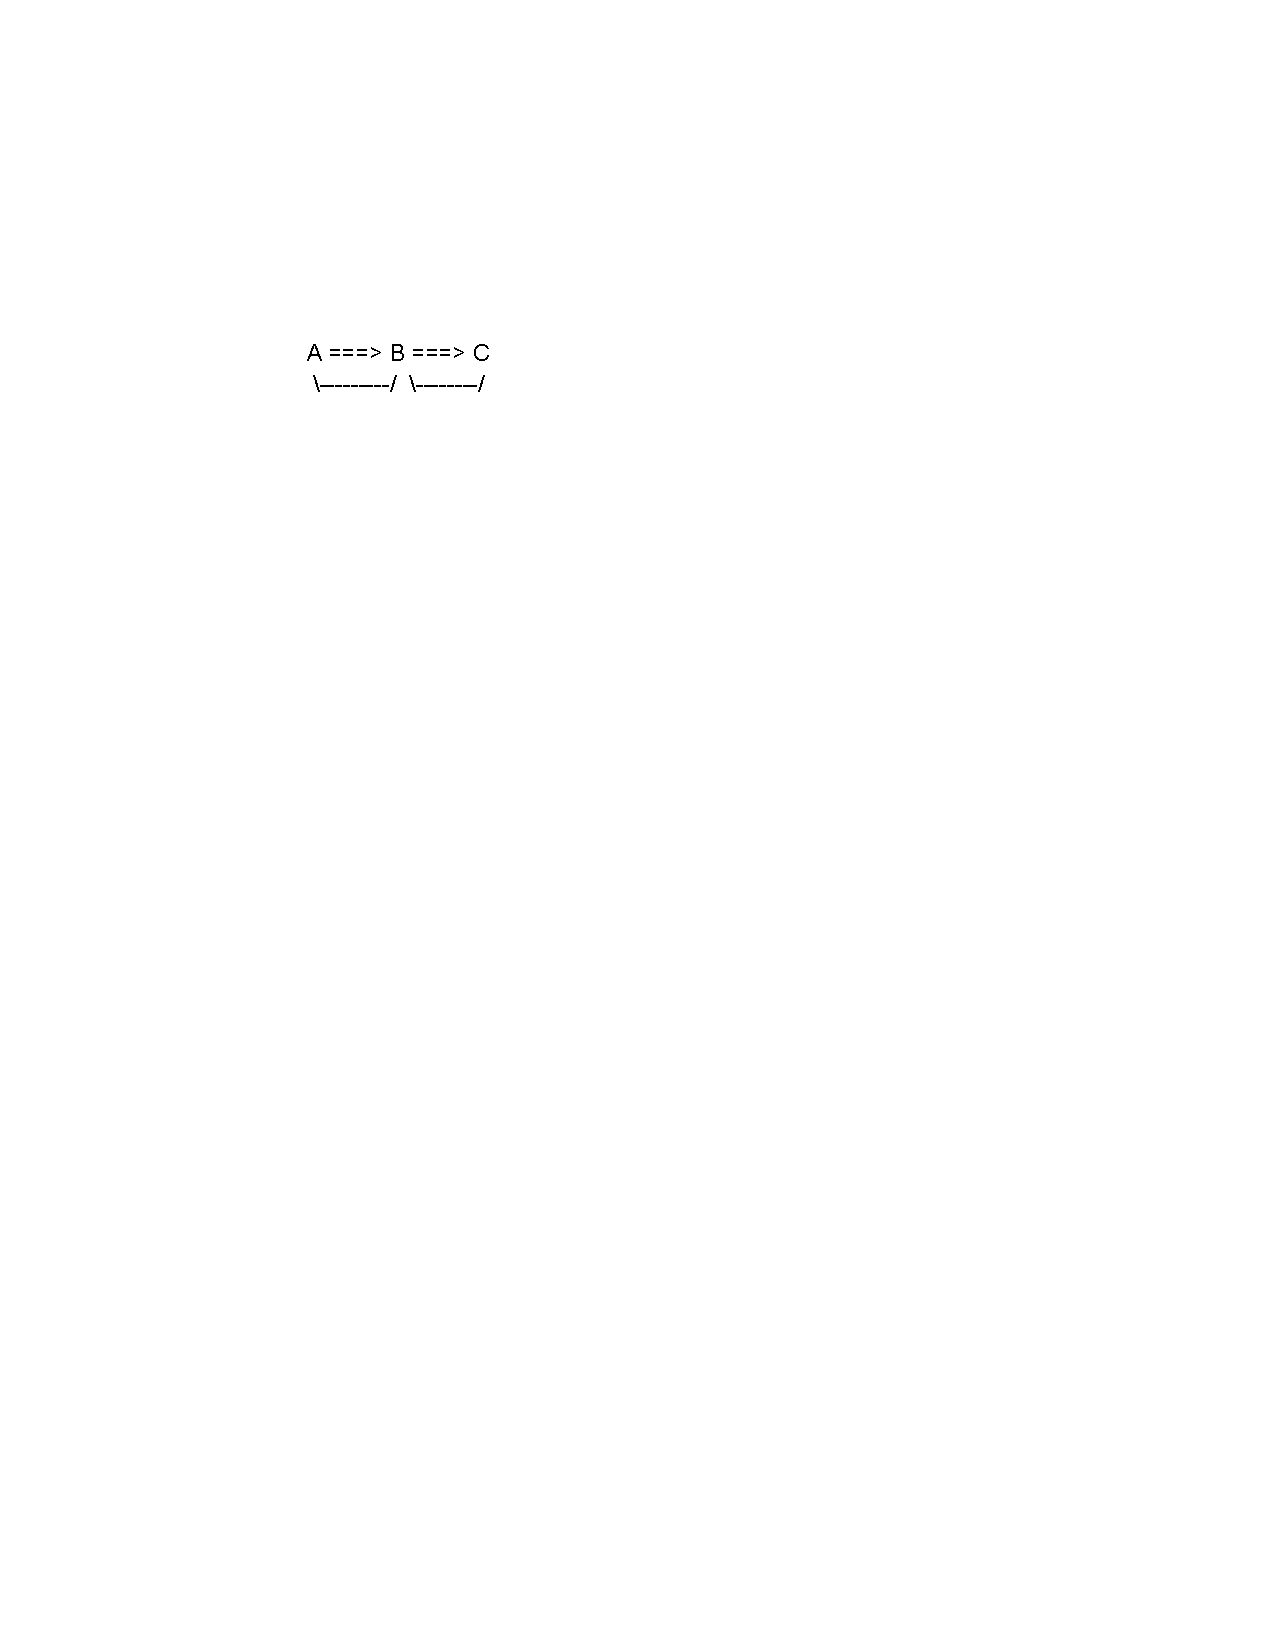
\includegraphics[]{figs/circular1}}
  \subfigure[case 2]{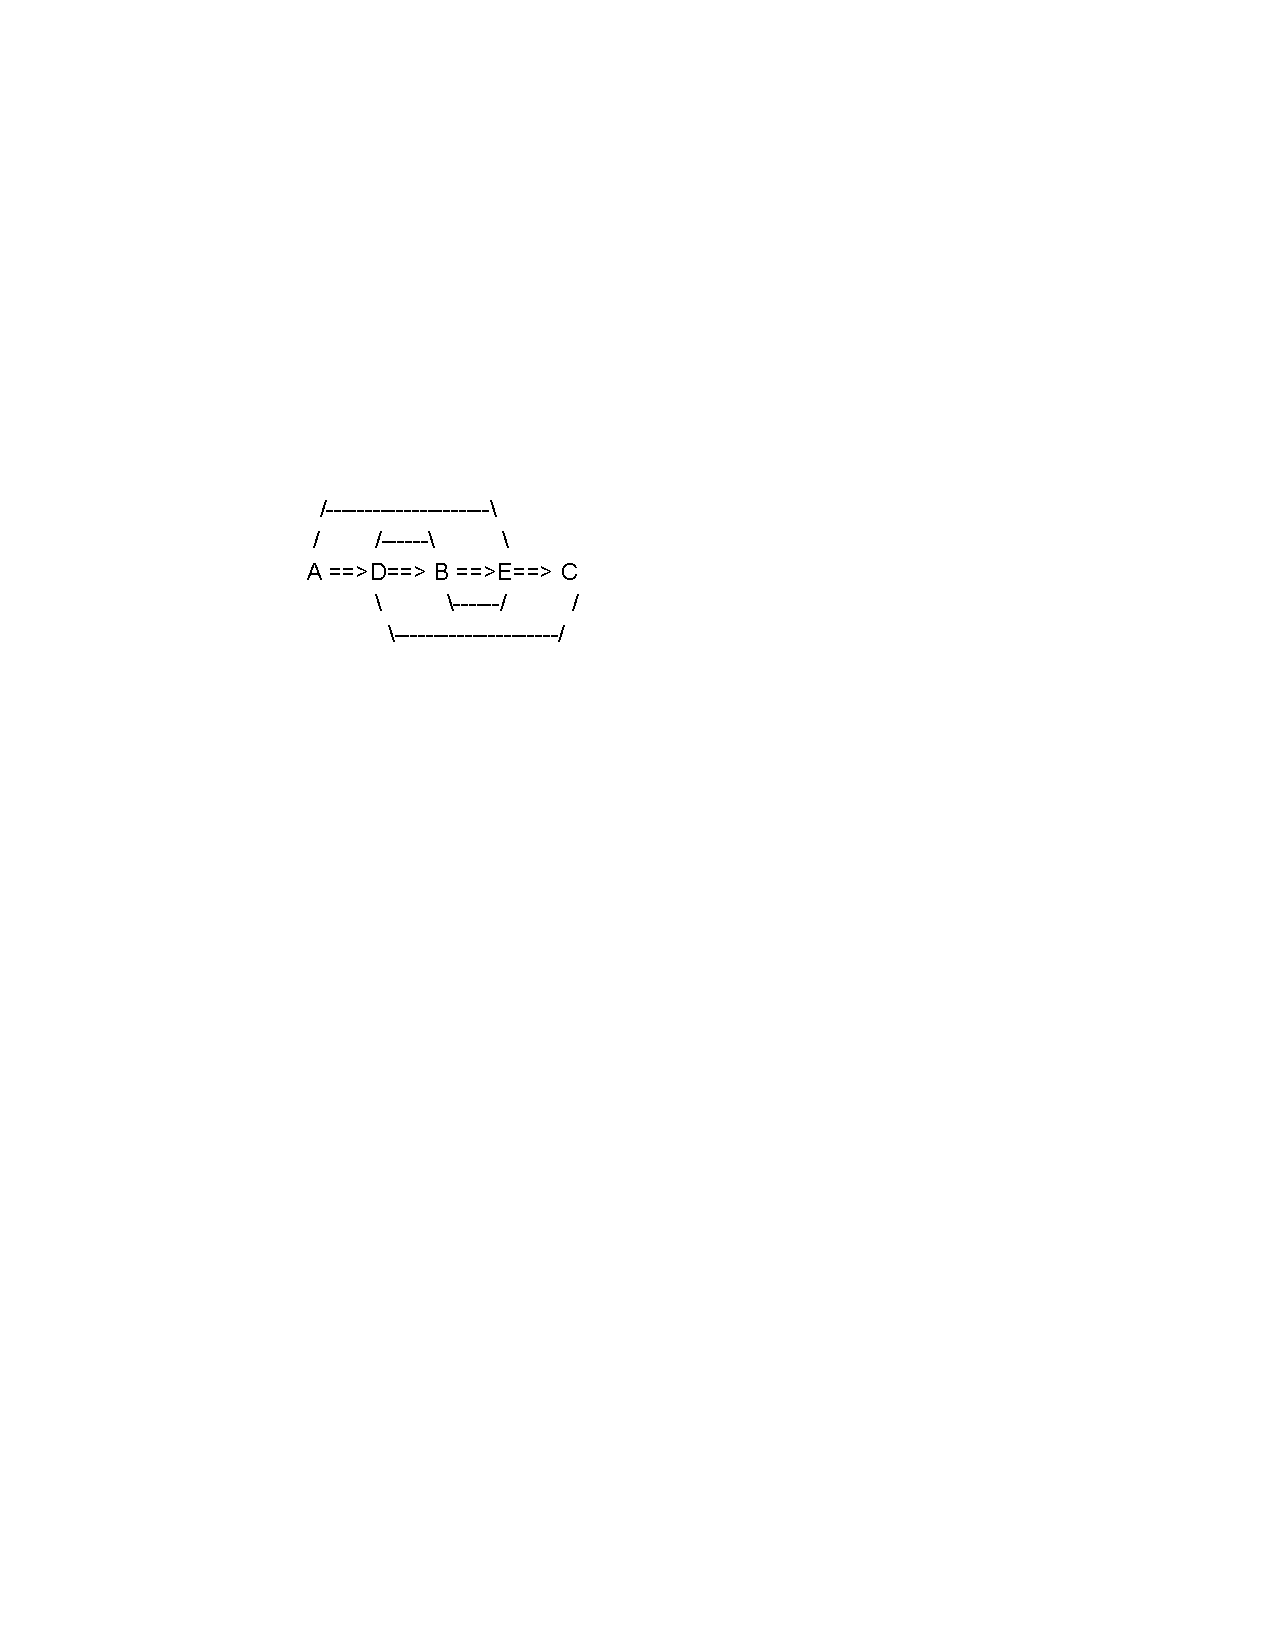
\includegraphics[]{figs/circular2}}
  \subfigure[case 3]{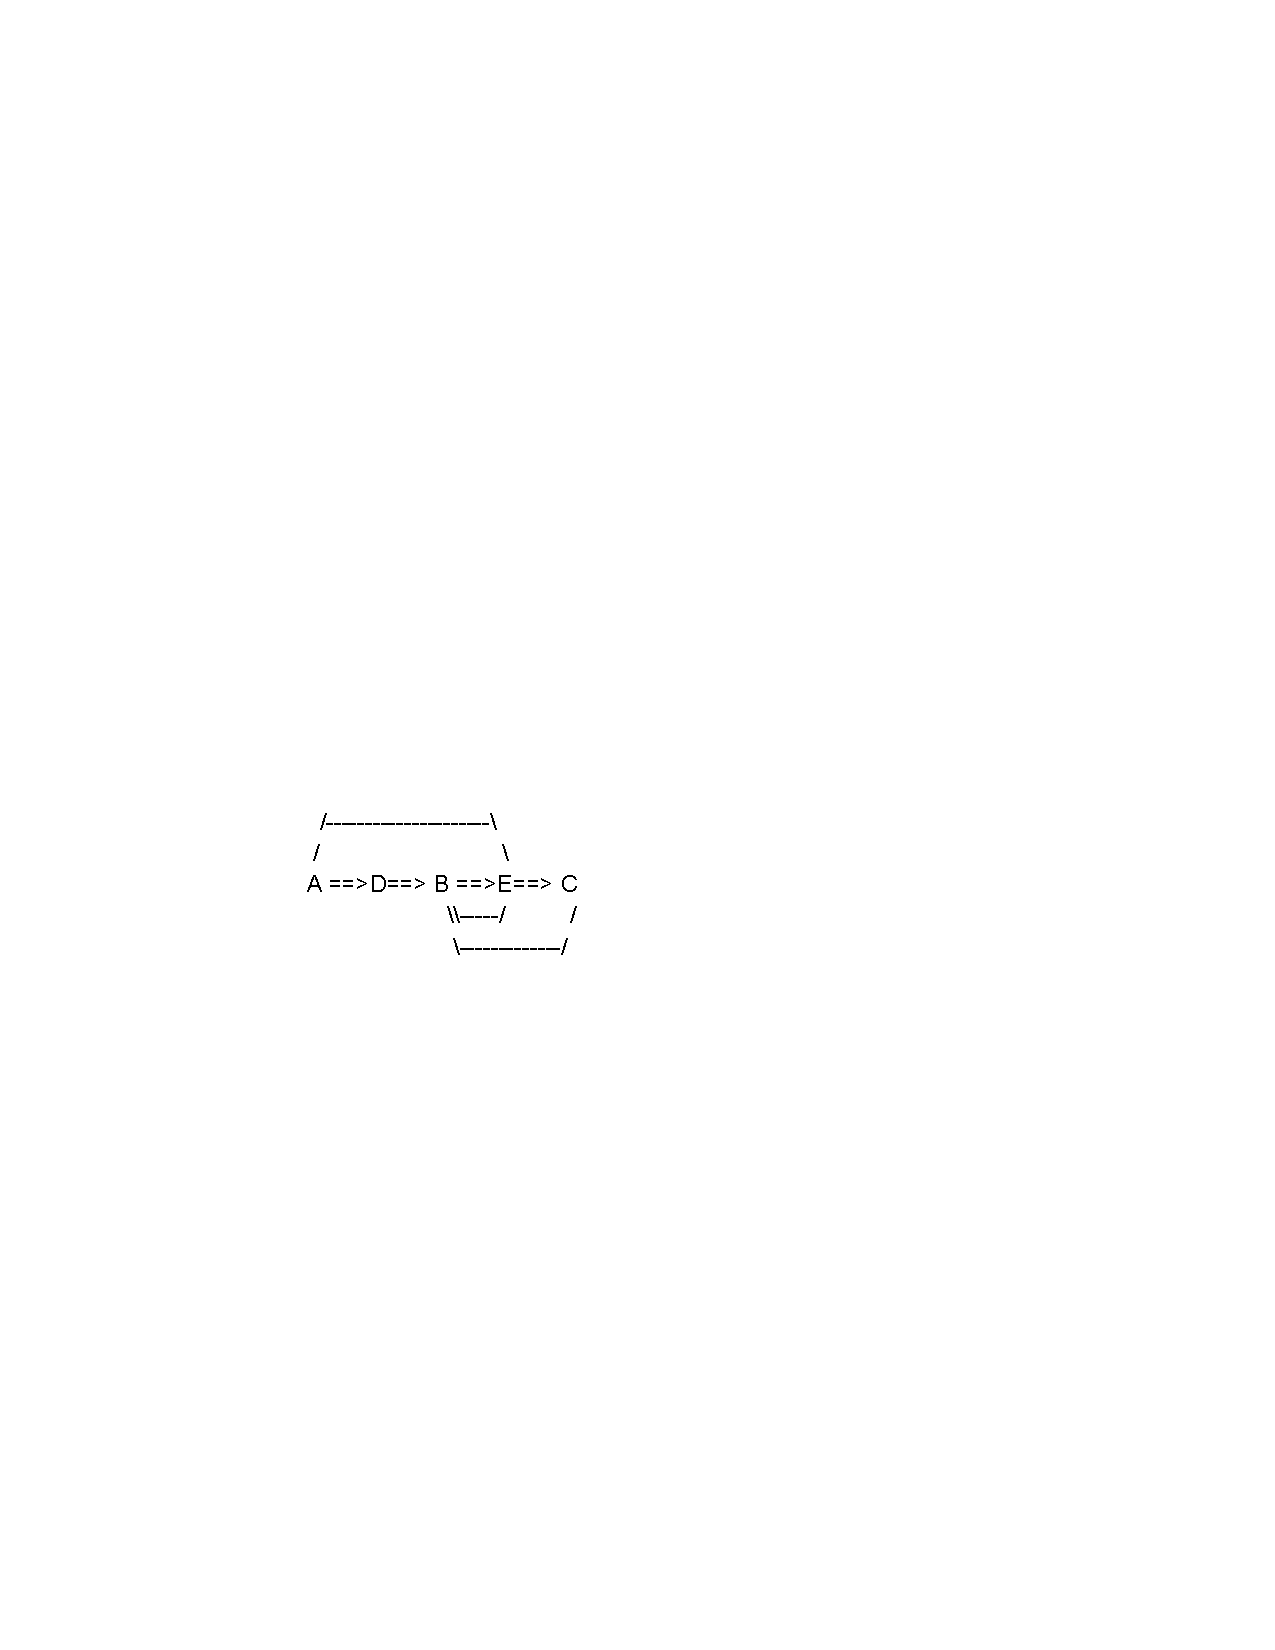
\includegraphics[]{figs/circular3}}
  \subfigure[case 4]{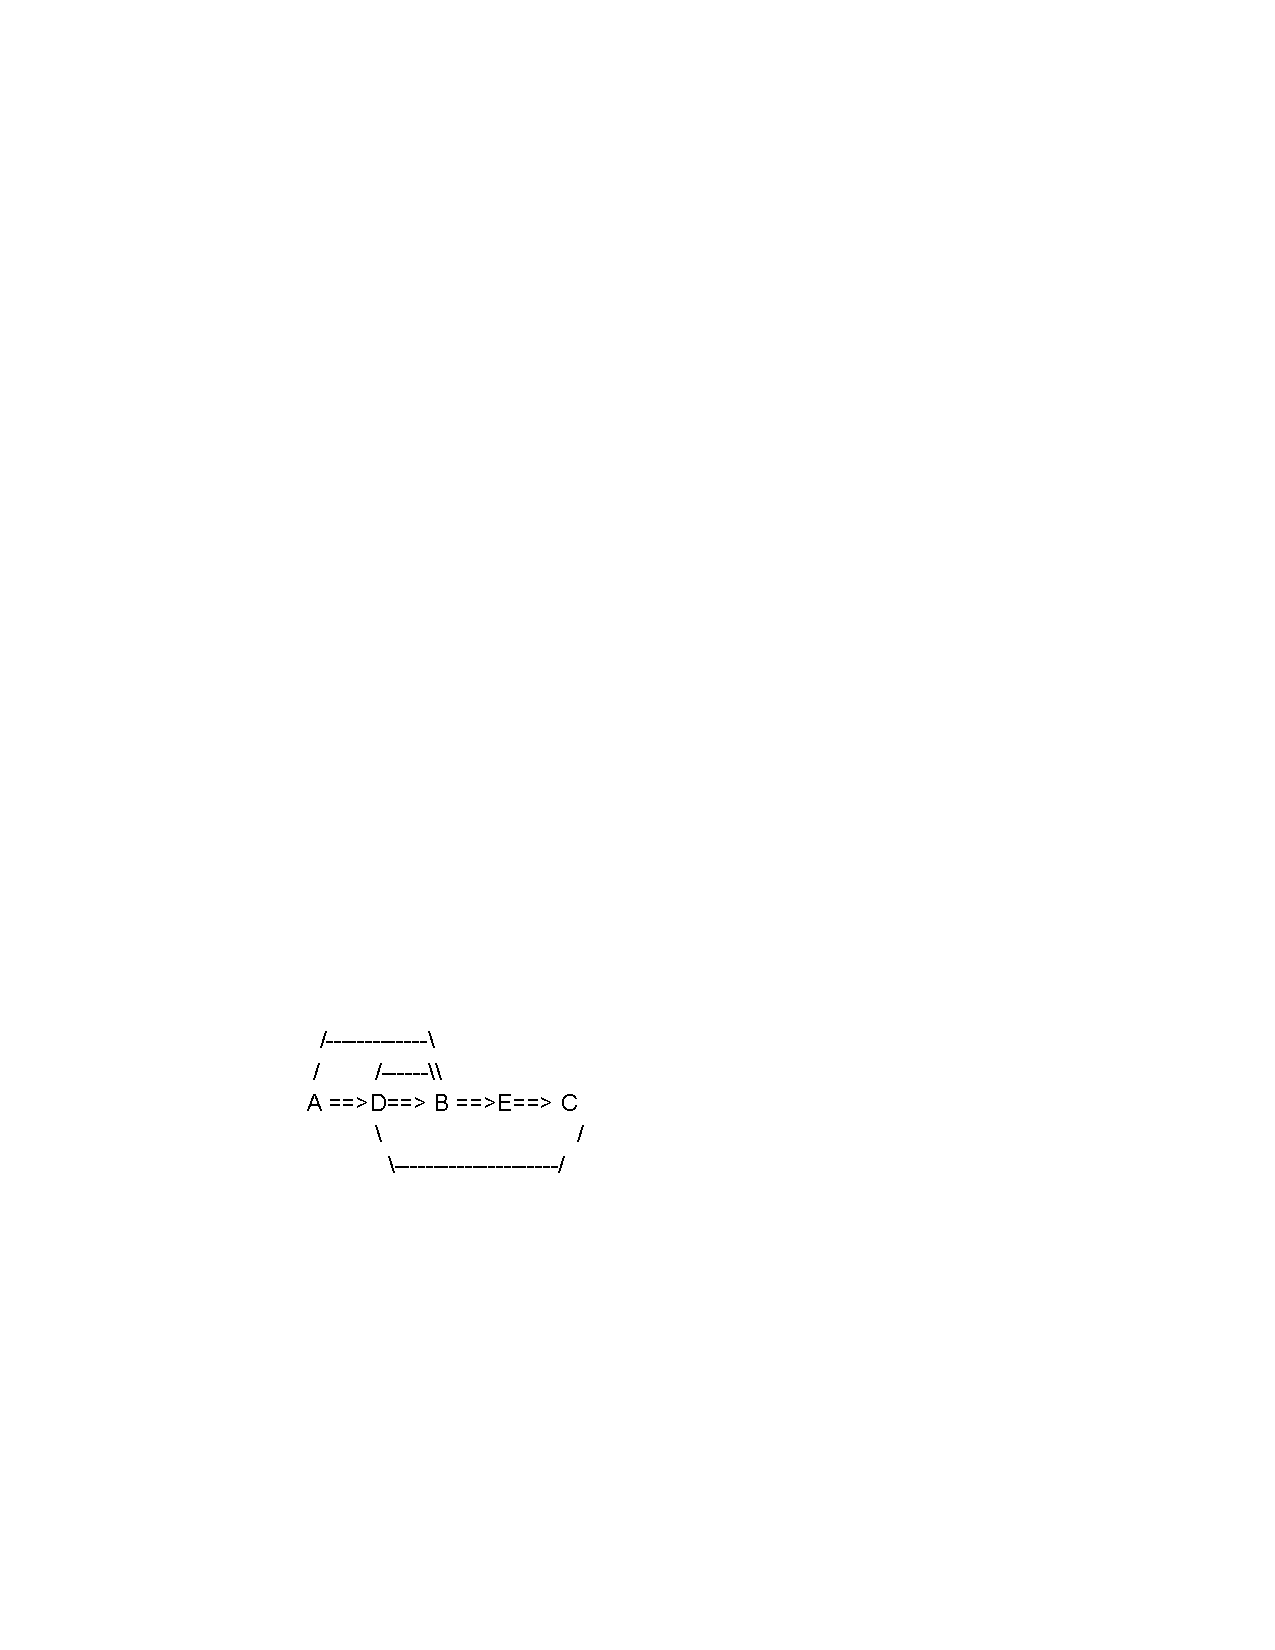
\includegraphics[]{figs/circular4}}
  \subfigure[case 5]{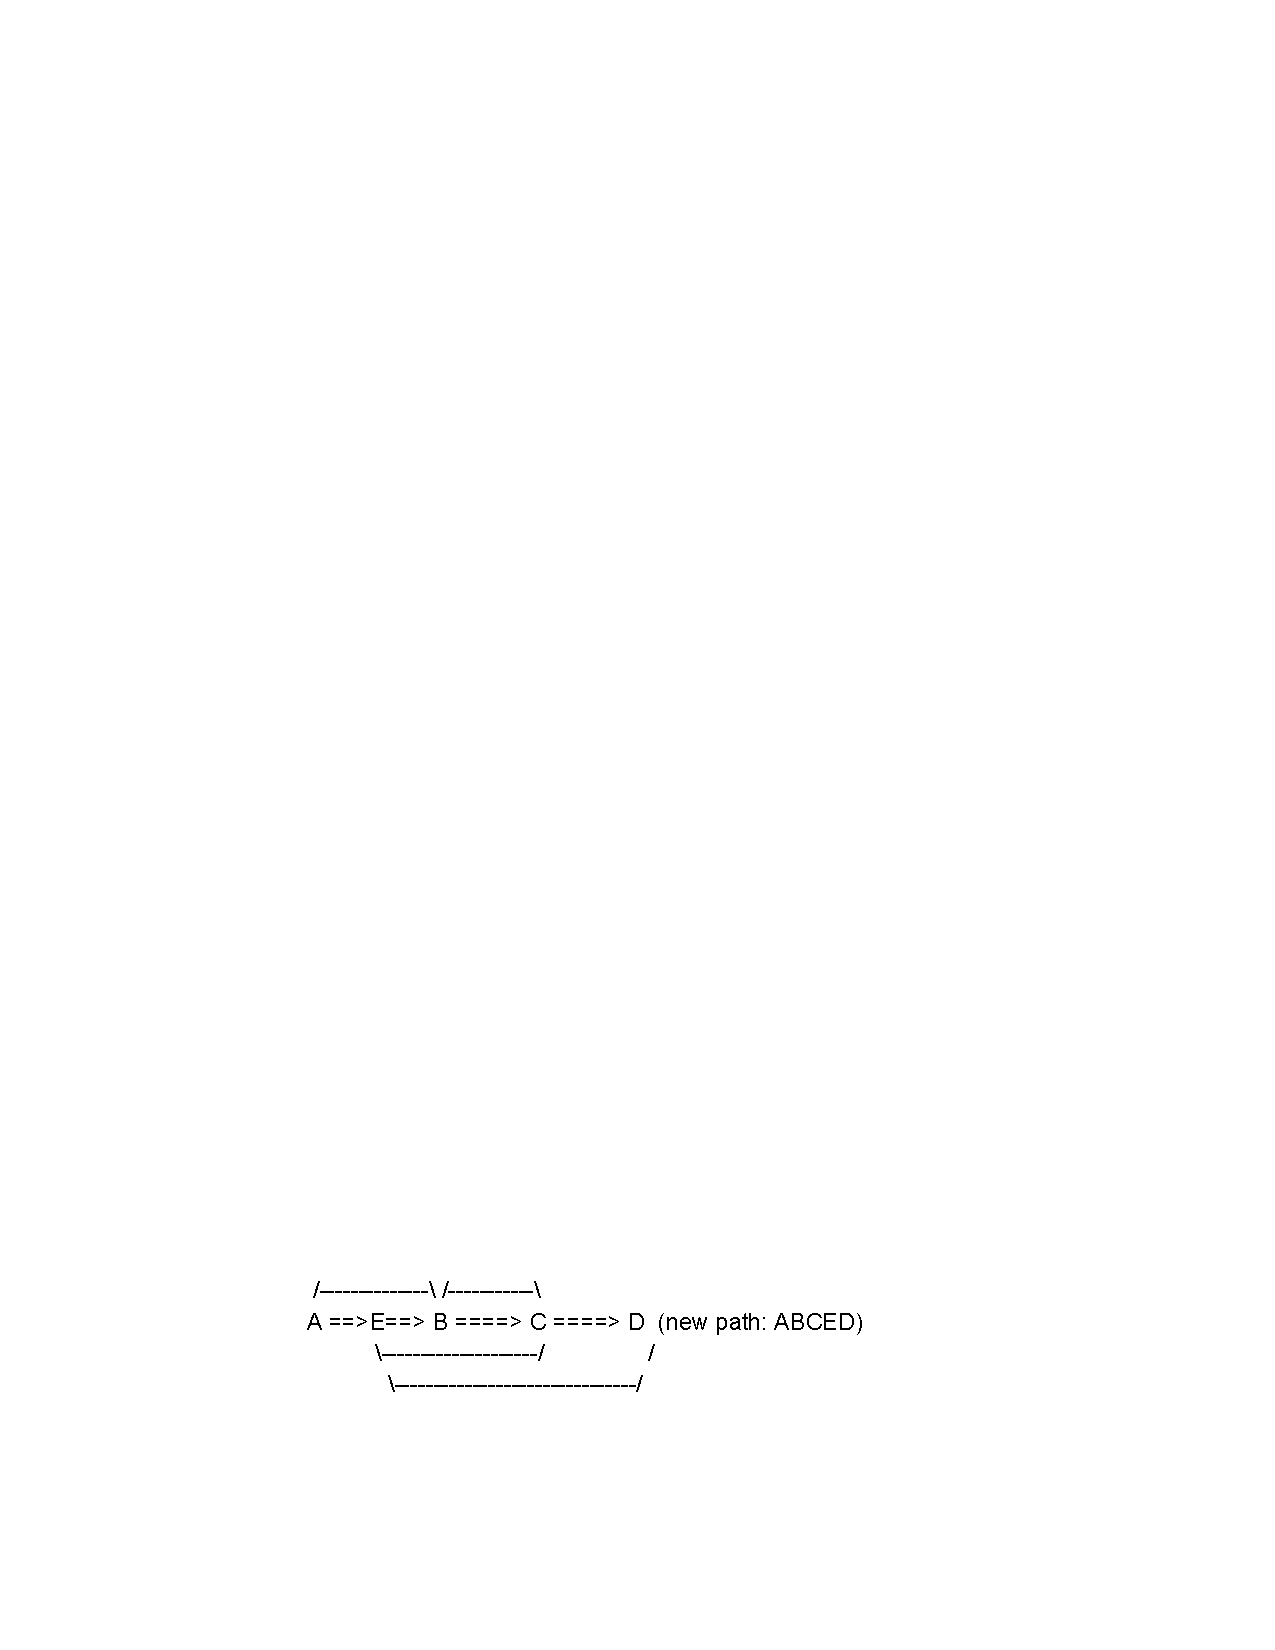
\includegraphics[]{figs/circular5}}
  %\vspace{10pt}
  \caption{\em \small Examples: circular dependencies between segments.}
  \label{fig:circular}
\end{figure}

\begin{theorem} (Conditions of the existence of an invariant complying update order): 
\begin{itemize}[noitemsep,topsep=0pt,leftmargin=*]
\item independent ECs, i.e., no overlapping updates across different ECs.
\item no circular dependencies between segments. 
In particular, if invariants are enforcing no more than two waypoints.
an update order always exists. 
\end{itemize} 
\end{theorem}

%\begin{proof}
%\end{proof}
\wxzc{need to prove it holds for multi-path?}

\paragraph{Other Categories?}

Overlapping ECs:
1. split updates to non-overlapping; 2. use mechanisms like consistent updates.

Slice isolation: If the output
of packet set of slice $a$ at any switch port, overlaps with any other slice,
then there is the potential for leaks. 

Multiple waypoints 

Path length constraint: Suppose
we wish to ensure that no flow from port $C$ to port $S$ should go through more
than 3 switches represents this check.

Quantitative properties (with SWAN)     
\fi                    
